\section{Date: 2026-07-29}
\noindent \textbf{Series ID: CWUR0000SAG} 

\noindent This series is titled Consumer Price Index for All Urban Wage Earners and Clerical Workers: Other Goods and Services in U.S. City Average and has a frequency of Monthly. The units are Index 1982-1984=100 and the seasonal adjustment is Not Seasonally Adjusted.The observation start date is 1967-01-01 and the observation end date is 2026-06-01.The popularity of this series is 2. \\ 

\noindent \textbf{Series ID: MESEPRPIHCSA} 

\noindent This series is titled Medical Services Expenditures by Provider Price Index and has a frequency of Annual. The units are Index 2017=100 and the seasonal adjustment is Not Seasonally Adjusted.The observation start date is 2000-01-01 and the observation end date is 2021-01-01.The popularity of this series is 3. \\ 

\subsection{Raw Regression}
\noindent Regresses the two series against each other directly. A significant result here can come just as easily from both series sharing a long-run trend as from any real relationship.

\begin{center}
\begin{tabular}{lclc}
\toprule
\textbf{Dep. Variable:}           & value\_fred\_MESEPRPIHCSA & \textbf{  R-squared:         } &     0.981   \\
\textbf{Model:}                   &            OLS            & \textbf{  Adj. R-squared:    } &     0.980   \\
\textbf{Method:}                  &       Least Squares       & \textbf{  F-statistic:       } &     1020.   \\
\textbf{Date:}                    &      Wed, 29 Jul 2026     & \textbf{  Prob (F-statistic):} &  1.23e-18   \\
\textbf{Time:}                    &          13:34:17         & \textbf{  Log-Likelihood:    } &   -48.503   \\
\textbf{No. Observations:}        &               22          & \textbf{  AIC:               } &     101.0   \\
\textbf{Df Residuals:}            &               20          & \textbf{  BIC:               } &     103.2   \\
\textbf{Df Model:}                &                1          & \textbf{                     } &             \\
\textbf{Covariance Type:}         &         nonrobust         & \textbf{                     } &             \\
\bottomrule
\end{tabular}
\begin{tabular}{lcccccc}
                                  & \textbf{coef} & \textbf{std err} & \textbf{t} & \textbf{P$> |$t$|$} & \textbf{[0.025} & \textbf{0.975]}  \\
\midrule
\textbf{const}                    &       4.9487  &        2.574     &     1.923  &         0.069        &       -0.421    &       10.318     \\
\textbf{value\_fred\_CWUR0000SAG} &       0.2061  &        0.006     &    31.936  &         0.000        &        0.193    &        0.220     \\
\bottomrule
\end{tabular}
\begin{tabular}{lclc}
\textbf{Omnibus:}       &  3.514 & \textbf{  Durbin-Watson:     } &    0.519  \\
\textbf{Prob(Omnibus):} &  0.173 & \textbf{  Jarque-Bera (JB):  } &    2.938  \\
\textbf{Skew:}          &  0.861 & \textbf{  Prob(JB):          } &    0.230  \\
\textbf{Kurtosis:}      &  2.512 & \textbf{  Cond. No.          } & 2.09e+03  \\
\bottomrule
\end{tabular}
%\caption{OLS Regression Results}
\end{center}

Notes: \newline
 [1] Standard Errors assume that the covariance matrix of the errors is correctly specified. \newline
 [2] The condition number is large, 2.09e+03. This might indicate that there are \newline
 strong multicollinearity or other numerical problems.

\begin{figure}
\centering
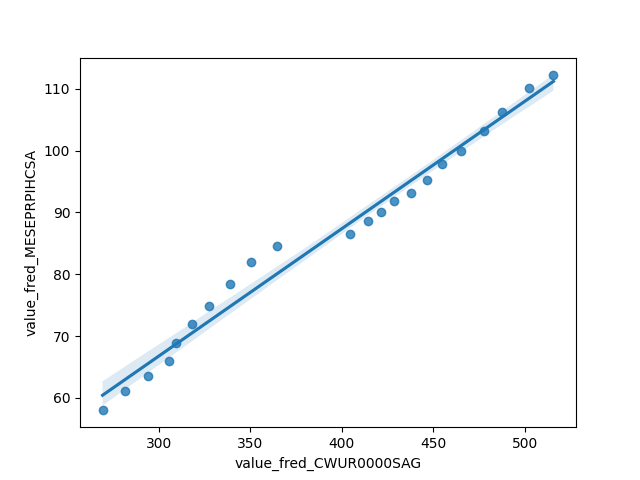
\includegraphics[scale = 0.9]{plots/plot_2026-07-29.png}
\caption{Raw Regression Plot for 2026-07-29}
\end{figure}
\newpage
\subsection{Detrended Regression}
\noindent Regresses the residuals of each series after removing its own linear time trend, so a shared trend can no longer drive the result on its own. A relationship that stays significant here is better evidence of a genuine link between the two series.

\begin{center}
\begin{tabular}{lclc}
\toprule
\textbf{Dep. Variable:}                      & value\_fred\_MESEPRPIHCSA\_detrended & \textbf{  R-squared:         } &     0.000   \\
\textbf{Model:}                              &                 OLS                  & \textbf{  Adj. R-squared:    } &    -0.050   \\
\textbf{Method:}                             &            Least Squares             & \textbf{  F-statistic:       } &  0.001018   \\
\textbf{Date:}                               &           Wed, 29 Jul 2026           & \textbf{  Prob (F-statistic):} &    0.975    \\
\textbf{Time:}                               &               13:34:17               & \textbf{  Log-Likelihood:    } &   -38.006   \\
\textbf{No. Observations:}                   &                    22                & \textbf{  AIC:               } &     80.01   \\
\textbf{Df Residuals:}                       &                    20                & \textbf{  BIC:               } &     82.19   \\
\textbf{Df Model:}                           &                     1                & \textbf{                     } &             \\
\textbf{Covariance Type:}                    &              nonrobust               & \textbf{                     } &             \\
\bottomrule
\end{tabular}
\begin{tabular}{lcccccc}
                                             & \textbf{coef} & \textbf{std err} & \textbf{t} & \textbf{P$> |$t$|$} & \textbf{[0.025} & \textbf{0.975]}  \\
\midrule
\textbf{const}                               &    1.002e-12  &        0.304     &  3.29e-12  &         1.000        &       -0.635    &        0.635     \\
\textbf{value\_fred\_CWUR0000SAG\_detrended} &      -0.0012  &        0.037     &    -0.032  &         0.975        &       -0.078    &        0.076     \\
\bottomrule
\end{tabular}
\begin{tabular}{lclc}
\textbf{Omnibus:}       &  2.786 & \textbf{  Durbin-Watson:     } &    0.239  \\
\textbf{Prob(Omnibus):} &  0.248 & \textbf{  Jarque-Bera (JB):  } &    1.903  \\
\textbf{Skew:}          &  0.527 & \textbf{  Prob(JB):          } &    0.386  \\
\textbf{Kurtosis:}      &  2.018 & \textbf{  Cond. No.          } &     8.25  \\
\bottomrule
\end{tabular}
%\caption{OLS Regression Results}
\end{center}

Notes: \newline
 [1] Standard Errors assume that the covariance matrix of the errors is correctly specified.

\begin{figure}
\centering
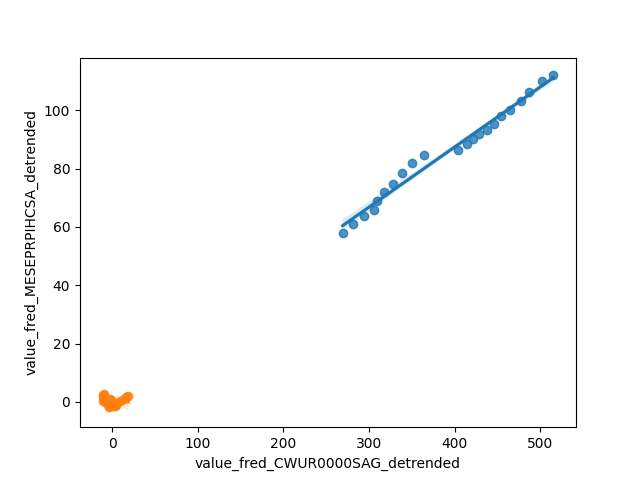
\includegraphics[scale = 0.9]{plots/plot_2026-07-29_detrended.png}
\caption{Detrended Regression Plot for 2026-07-29}
\end{figure}
\newpage
